This section describes the application layer, the uppermost layer presented in Figure \ref{fig:datastack}, which takes advantage of the data stack described above. The software described is the Hopsworks feature store, which this project contributes to. This software is part of the broader \gls{MLOps} platform offered by Hopsworks AB, the company that hosted this master thesis.


\subsection{Machine Learning Operations (MLOps)}
\label{subsec:back_mlops}

\gls{MLOps} are a full set of practices related to the development and automation of \gls{ML} workflows. Through the \gls{MLOps} lenses, a \gls{ML} workflow is logically separated in smaller steps, and considered from a data, code and model perspective. Differently from a classical software application, where only the code needs versioning, in the context of \gls{ML} applications, it is key that all three of data, code and model are versioned. Perhaps, different data might be used by models in different moments, as well as new model might be trained on the same data, to truly understand their improvements.The novel challenges are thus related to data validation, \gls{ML} artifacts versioning, \gls{ML} workflow orchestration, and infrastructure management, given higher computation and storage capabilities needed by those workflows \cite{SurgeAI2024,PDFBigData2024}.

The need of the described features saw new solutions emerging, like the Hopsworks AI data platform \cite{HopsworksRealtimeAI}. In the context of data versioning, the specific solution is called feature store \cite{MeetMichelangeloUbers2017}, which consists in a centralized fast-access storage for both real-time and batch data.

A simple architecture following \gls{MLOps} principle is presented in Figure \ref{fig:mlops_hops}. As first step, data are gathered either streaming (real-time) or batch data sources. A feature pipeline process those the data, performing model-independent transformations \cite{BigDictionaryMLOps2024}, and saves them in the feature store. A training pipeline runs now model-dependent transformations on features and labels retrieved from the feature store, and train the respective model, saving the trained model in the model registry. The last pipeline, the inference pipeline, extract at its need a specific model from the model registry and access the features, over which a inference will be conducted, from the feature store. The output of this pipeline, which normally is embedded directly in the consuming application, are the predictions of the model over the selected features, altogether with logs describing the performance of the model according to a pre-selected measure. All the pipeline are decoupled and could thus work asynchronously, making the whole \gls{ML} workflow scalabile, maintainable and effective.

\begin{figure}[!ht]
    \begin{center}
      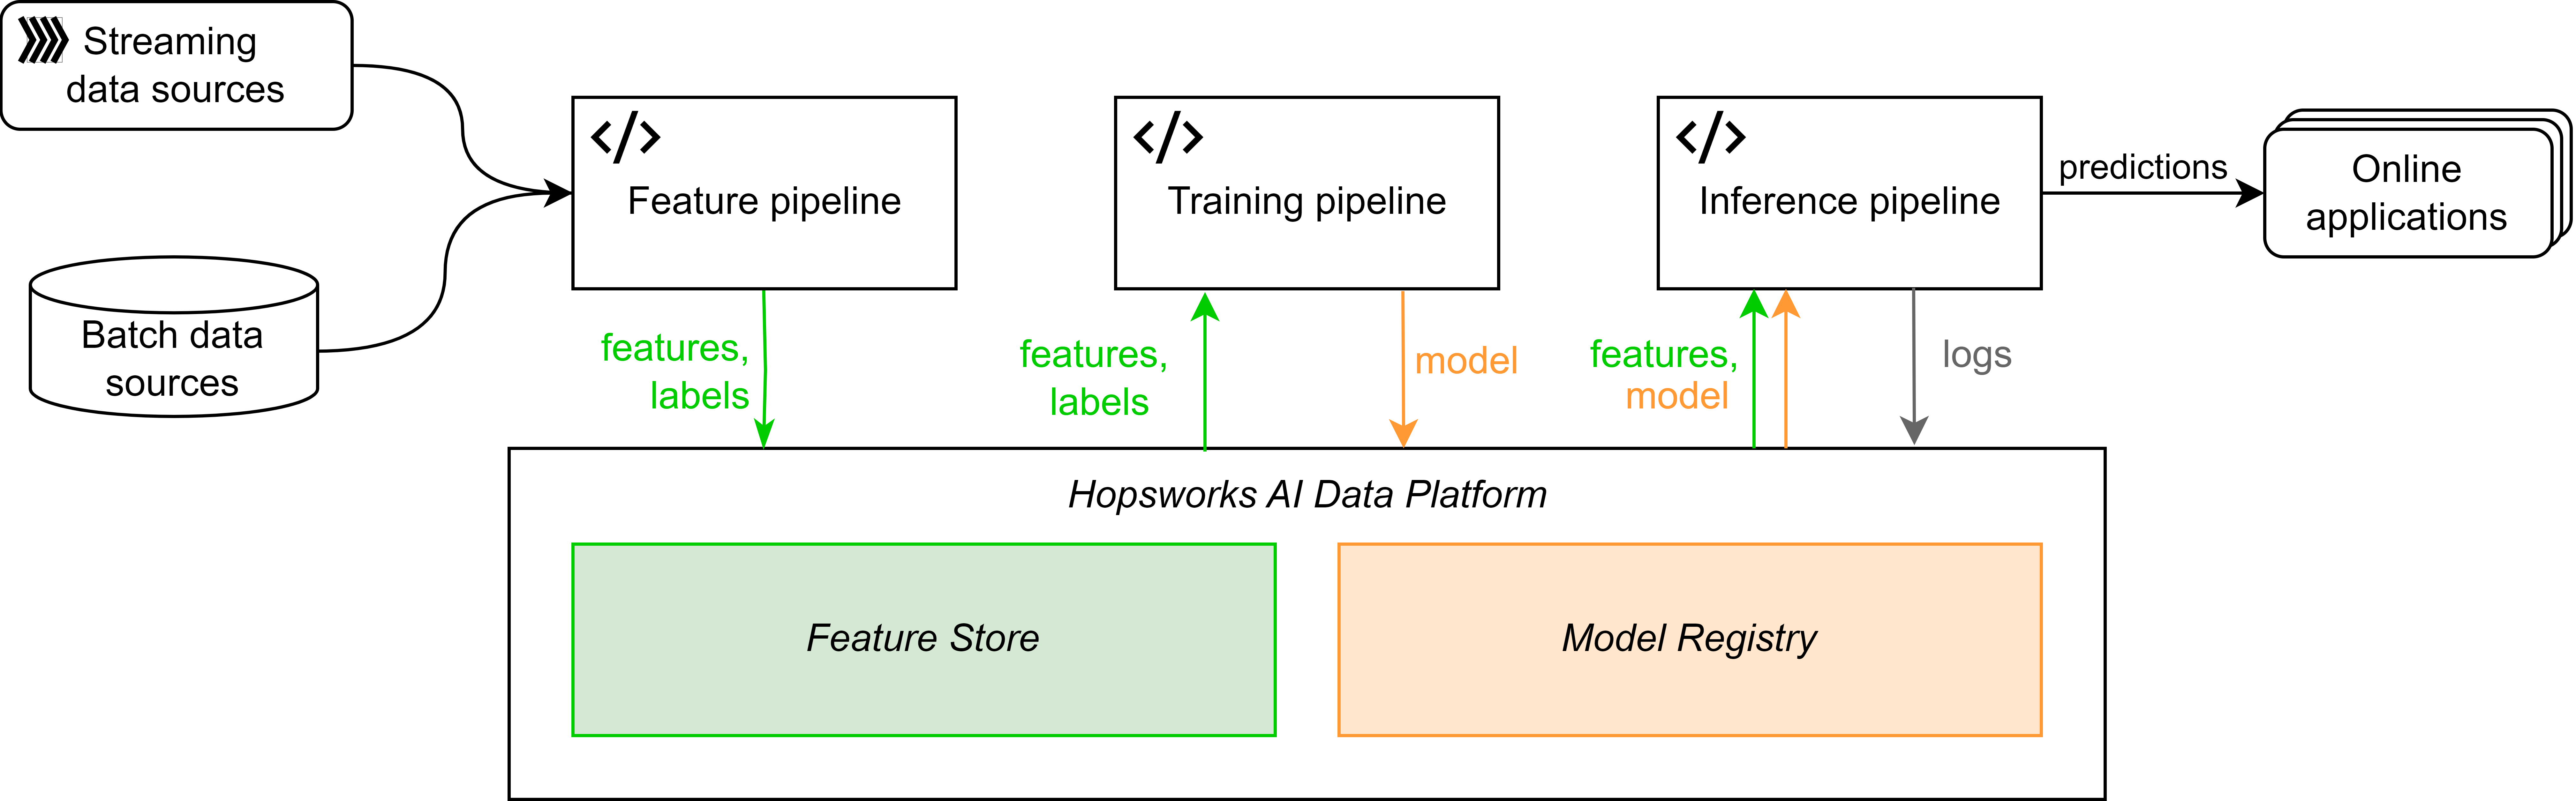
\includegraphics[width=\textwidth]{figures/2-background_and_related_work/MLOps_hops.png}
    \end{center}
    \caption[Feature store in an MLOps pipeline]{\glstext{MLOps} pipeline using a feature store and a model registry. Diagram inspired by Hopsworks documentation available at \url{https://www.hopsworks.ai/dictionary/feature-store}.}
    \label{fig:mlops_hops}
\end{figure}


\subsection{Hopsworks AI Data Platform}
\label{subsec:back_hopsworks_FS}
As briefly said above, the feature Store is a key data layer in an \gls{ML} application built over the \gls{MLOps} principles. The feature store enables feature reusability, as well as multi-user collaboration and a centralized authenticated access to the feature. The Hopsworks feature store organizes features in feature groups. Those are mutable collection of features, over which developers can perform \gls{CRUD} operations, accessing them via the Hopsworks \glspl{API}.

The Hopsworks feature store supports both batch data sources and real-time data streaming. This hybrid system is possible thanks to the dual implementation of an offline and an offline feature store. The offline feature store is a column-based storage suited for batch data that is updated with a low frequency (every few hours at maximum frequency). The online feature store, on the other hand, is a real-time row-based, key-value data storage based on RonDB, thus enabling low latency and real-time processing. To maintain consistentency between those two stacks, the Hopsworks feature store has a unique point of entry for data, which is Kafka, explained in detail in \ref{subsec:back_apache_kafka}. This guarantess that each message is delivered to both storages, which acts are consumers subscribed to the Kafka topics.

The model registry works under the same principles of the feature store, proving a centralized access and a standard deployment for all the models saved in it. It also saves information about model performance along time, model schemas and training feature logs, to ease model reproducibility and tracking.